%\section {Random methods}

%
% History
%

\begin{frame}{History}
  \begin{itemize}
  \item Before the 1990's: mainly a mathematical problem
    \begin{itemize}
    \item real algebraic geometry,
    \item decidability: Schwartz and Sharir 1982,
      \begin{itemize}
      \item Tarski theorem, Collins decomposition,
      \end{itemize}
    \end{itemize}
    \pause
  \item from the 1990's: an algorithmic problem
    \begin{itemize}
    \item random sampling (1993),
    \item asymptotically optimal random sampling (2011).
    \end{itemize}
  \end{itemize}
\end{frame}
%
%  random methods
%

\begin{frame} {Random methods}
  \begin{itemize}
  \item In the early 1990's, random methods started being developed
    \pause
  \item Principle
    \begin{itemize}
    \item shoot random configurations
      \pause
    \item test whether they are in collision
      \pause
    \item build a graph (roadmap)  the nodes of which are free configurations
      \pause
    \item  and the edges of which are collision-free linear interpolations
    \end{itemize}
  \end{itemize}
\end{frame}

%
%  La méthode des arbres aléatoires d'exploration rapide.
%

\begin{frame} {Rapidly exploring Random Tree (RRT) 2000}
\centerline {
  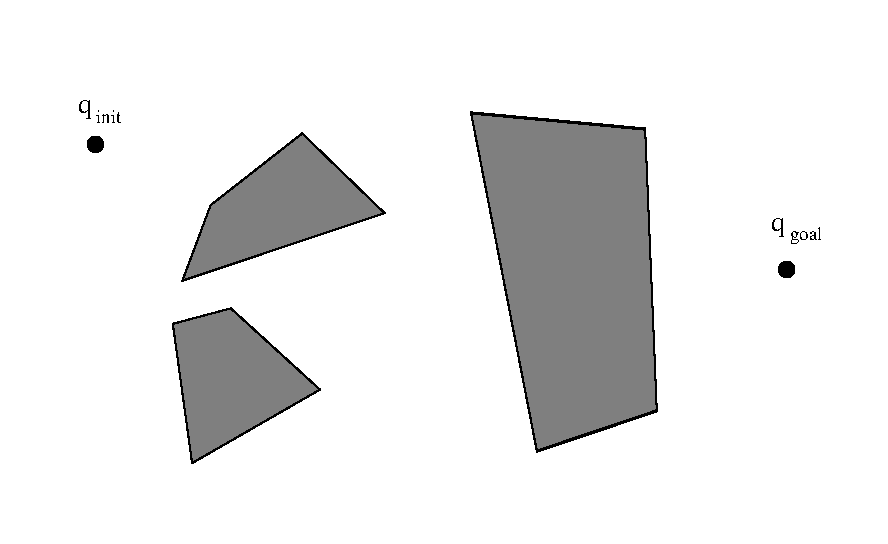
\includegraphics[width=.8\linewidth]{figures/RRT00.pdf}
}
\end{frame}

\begin{frame} {Rapidly exploring Random Tree (RRT) 2000}
\centerline {
  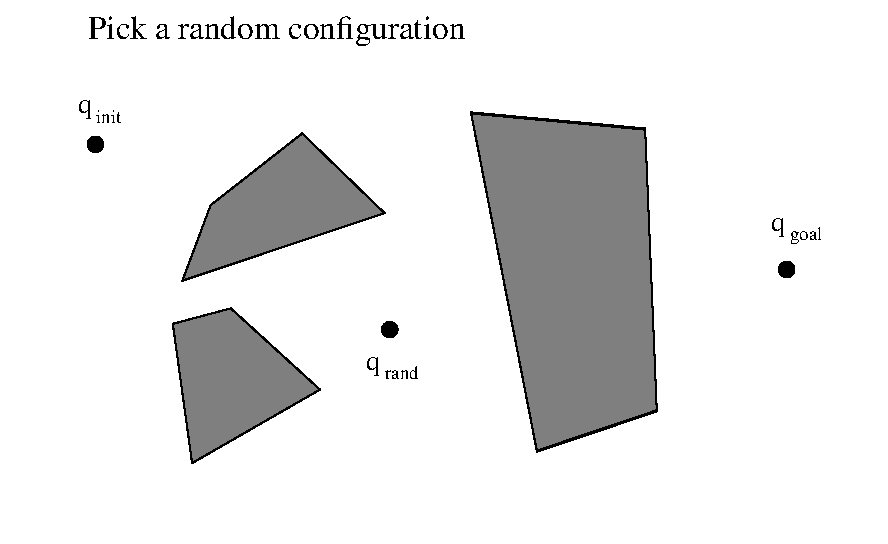
\includegraphics[width=.8\linewidth]{figures/RRT01.pdf}
}
\end{frame}

\begin{frame} {Rapidly exploring Random Tree (RRT) 2000}
\centerline {
  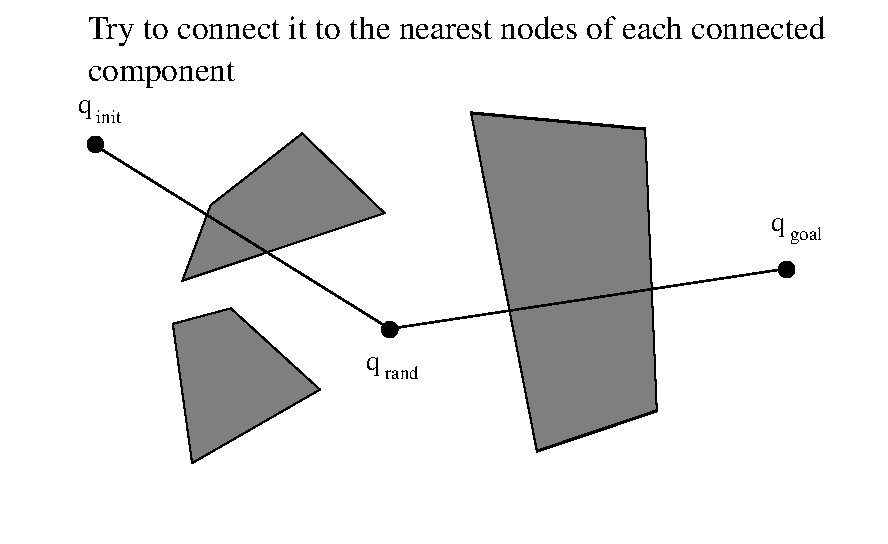
\includegraphics[width=.8\linewidth]{figures/RRT02.pdf}
}
\end{frame}

\begin{frame} {Rapidly exploring Random Tree (RRT) 2000}
\centerline {
  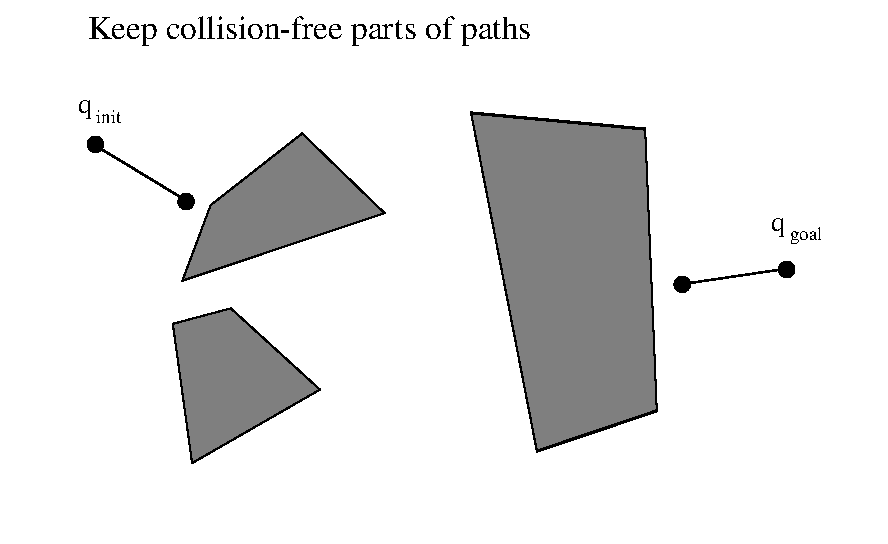
\includegraphics[width=.8\linewidth]{figures/RRT04.pdf}
}
\end{frame}

\begin{frame} {Rapidly exploring Random Tree (RRT) 2000}
\centerline {
  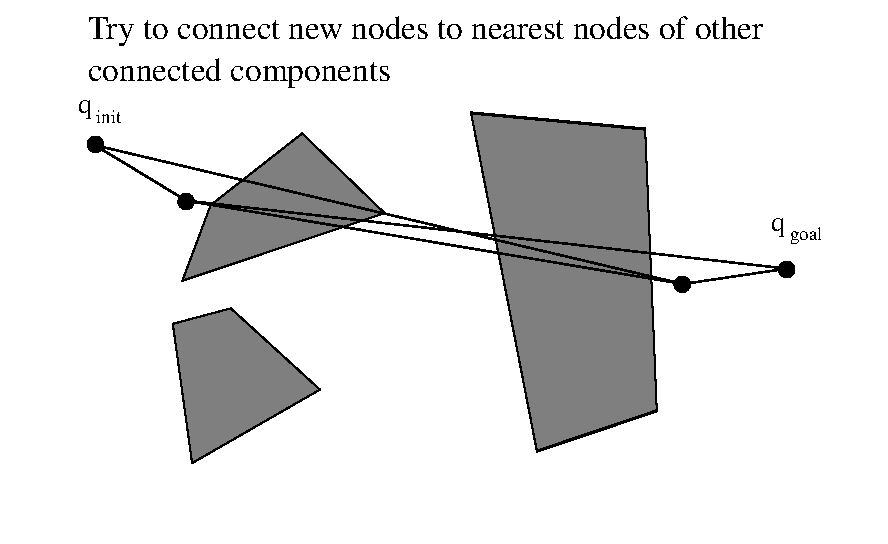
\includegraphics[width=.8\linewidth]{figures/RRT05.pdf}
}
\end{frame}

\begin{frame} {Rapidly exploring Random Tree (RRT) 2000}
\centerline {
  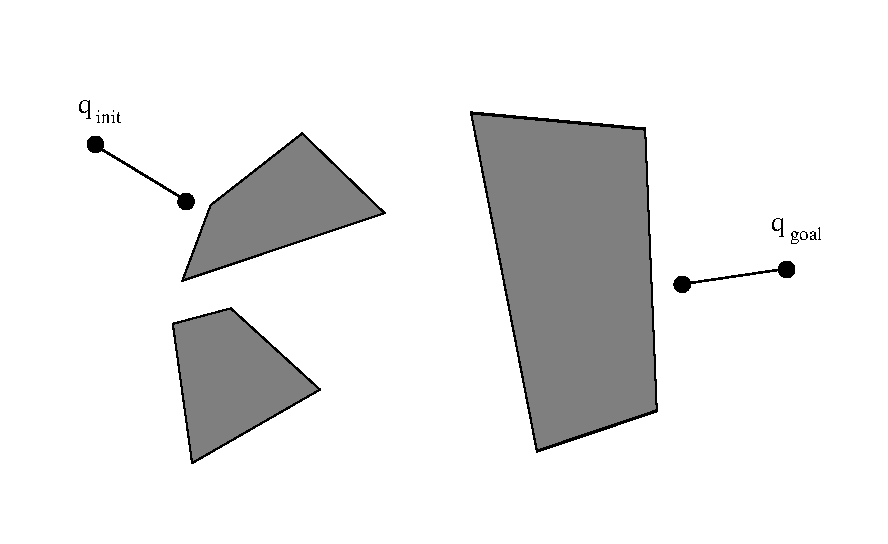
\includegraphics[width=.8\linewidth]{figures/RRT06.pdf}
}
\end{frame}

\begin{frame} {Rapidly exploring Random Tree (RRT) 2000}
\centerline {
  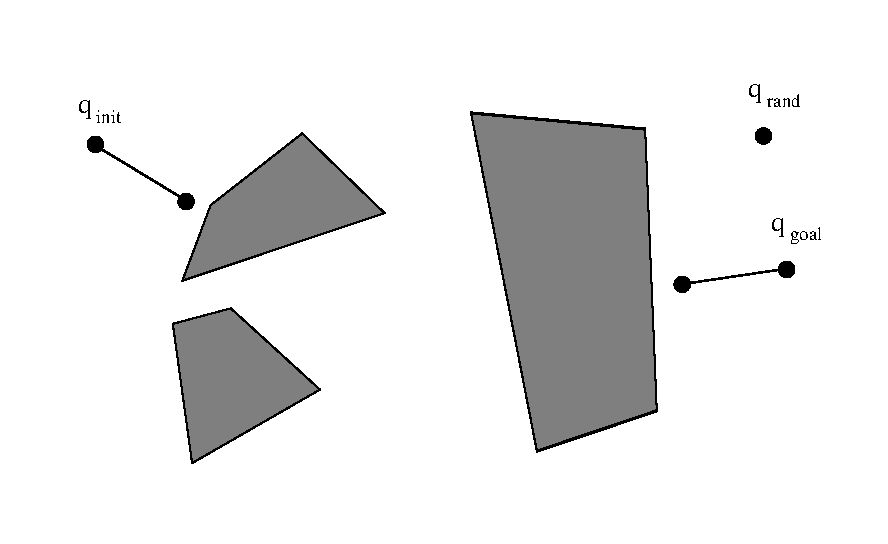
\includegraphics[width=.8\linewidth]{figures/RRT07.pdf}
}
\end{frame}

\begin{frame} {Rapidly exploring Random Tree (RRT) 2000}
\centerline {
  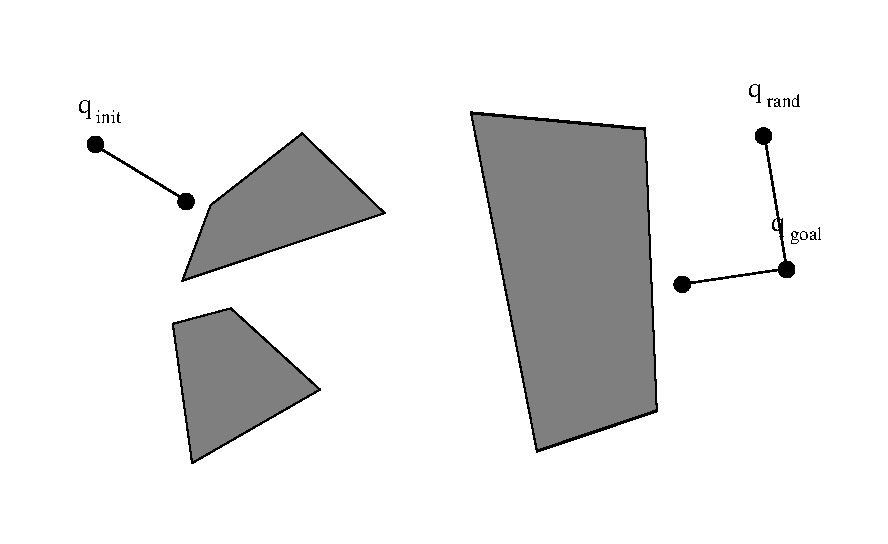
\includegraphics[width=.8\linewidth]{figures/RRT08.pdf}
}
\end{frame}

\begin{frame} {Rapidly exploring Random Tree (RRT) 2000}
\centerline {
  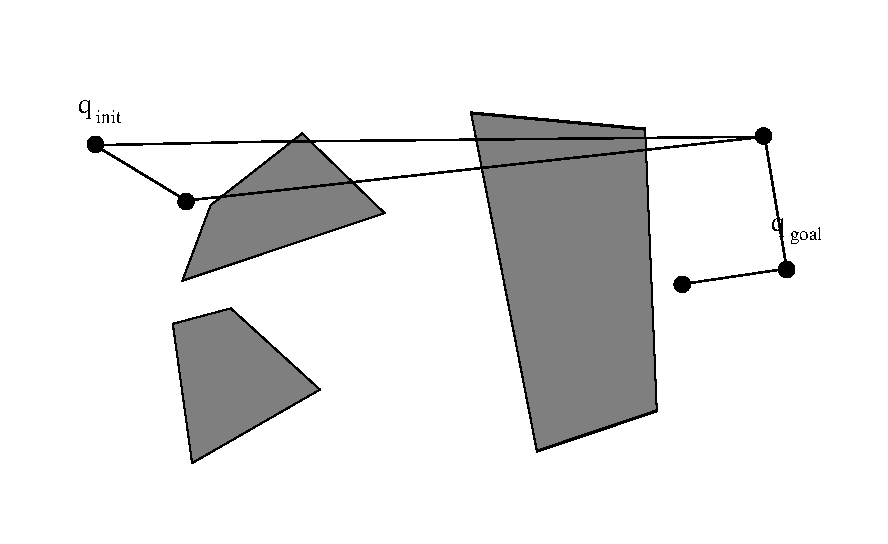
\includegraphics[width=.8\linewidth]{figures/RRT09.pdf}
}
\end{frame}

\begin{frame} {Rapidly exploring Random Tree (RRT) 2000}
\centerline {
  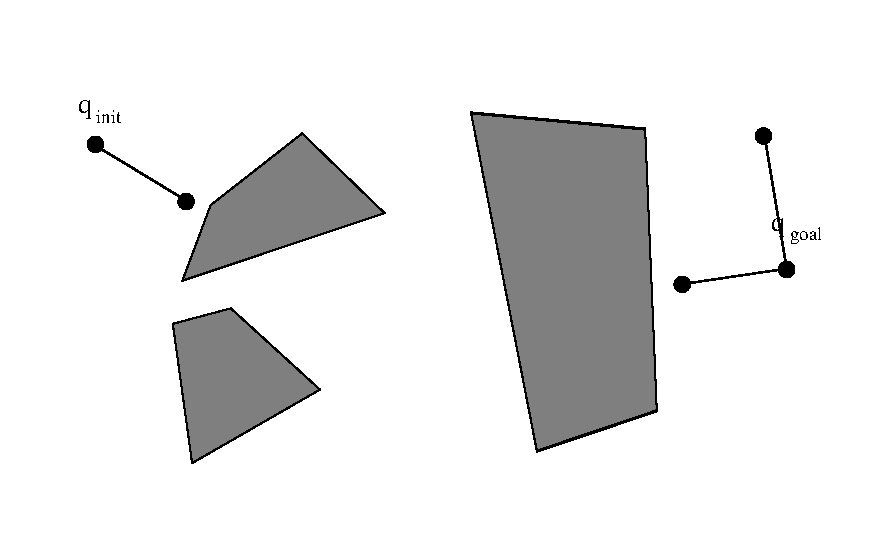
\includegraphics[width=.8\linewidth]{figures/RRT10.pdf}
}
\end{frame}

\begin{frame} {Rapidly exploring Random Tree (RRT) 2000}
\centerline {
  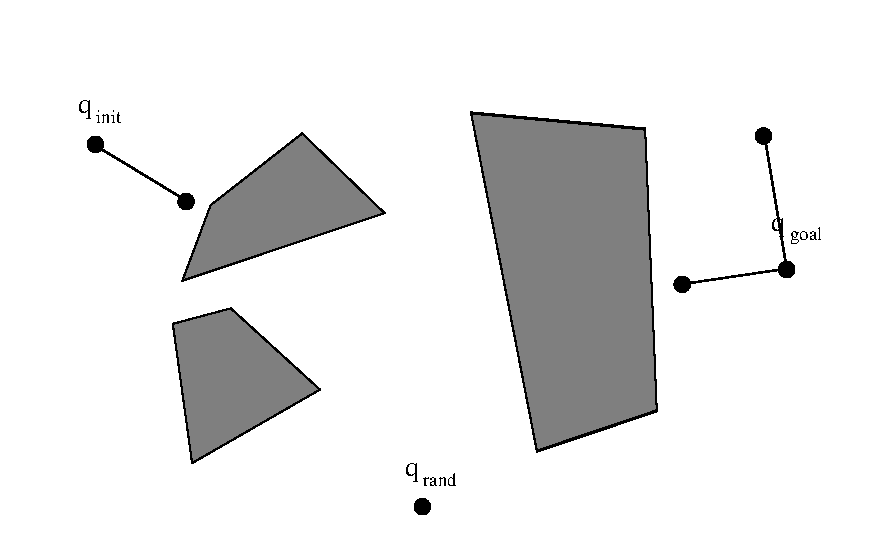
\includegraphics[width=.8\linewidth]{figures/RRT11.pdf}
}
\end{frame}

\begin{frame} {Rapidly exploring Random Tree (RRT) 2000}
\centerline {
  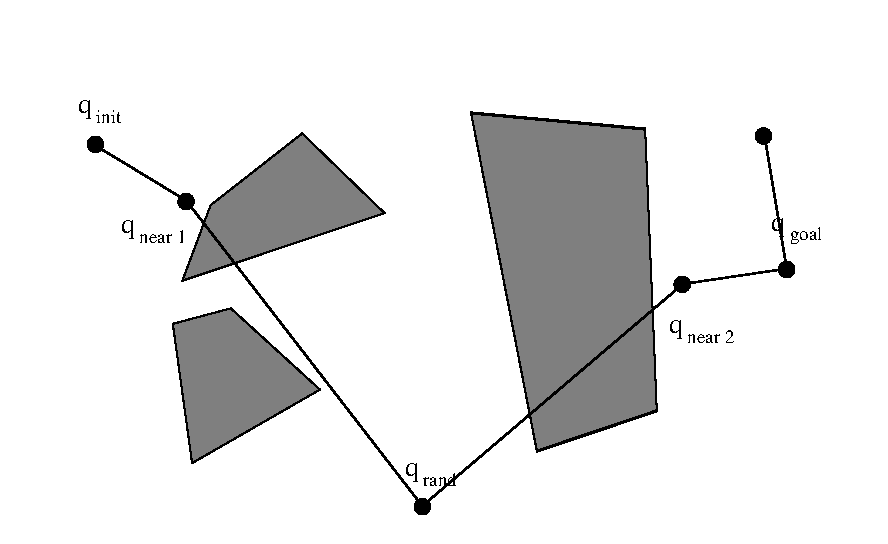
\includegraphics[width=.8\linewidth]{figures/RRT12.pdf}
}
\end{frame}

\begin{frame} {Rapidly exploring Random Tree (RRT) 2000}
\centerline {
  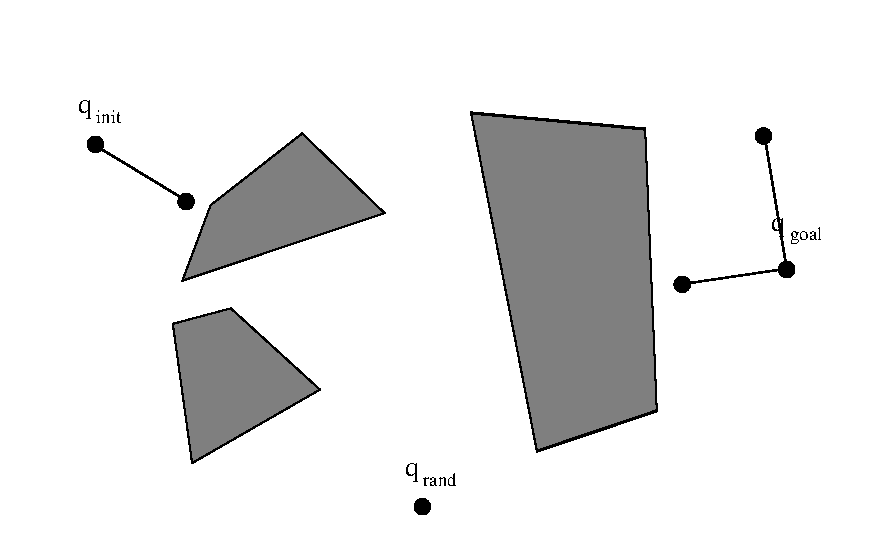
\includegraphics[width=.8\linewidth]{figures/RRT13.pdf}
}
\end{frame}

\begin{frame} {Rapidly exploring Random Tree (RRT) 2000}
\centerline {
  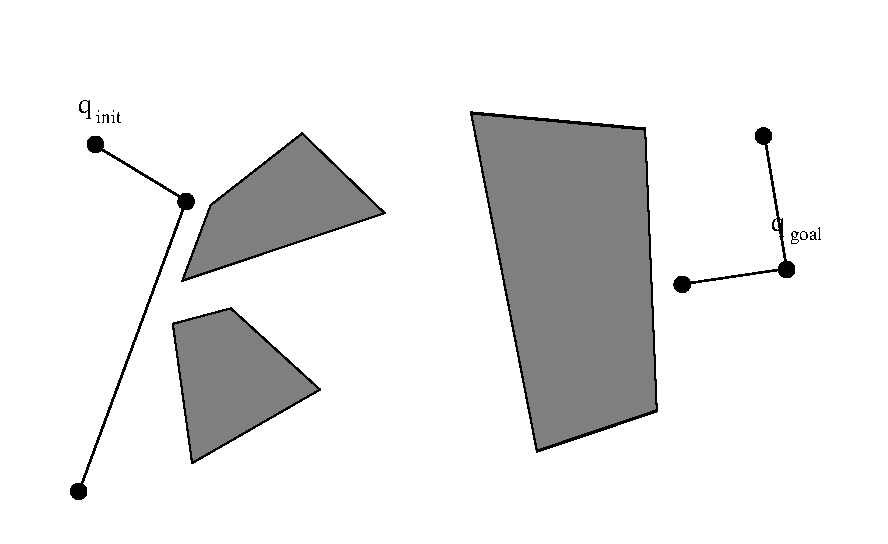
\includegraphics[width=.8\linewidth]{figures/RRT14.pdf}
}
\end{frame}

\begin{frame} {Rapidly exploring Random Tree (RRT) 2000}
\centerline {
  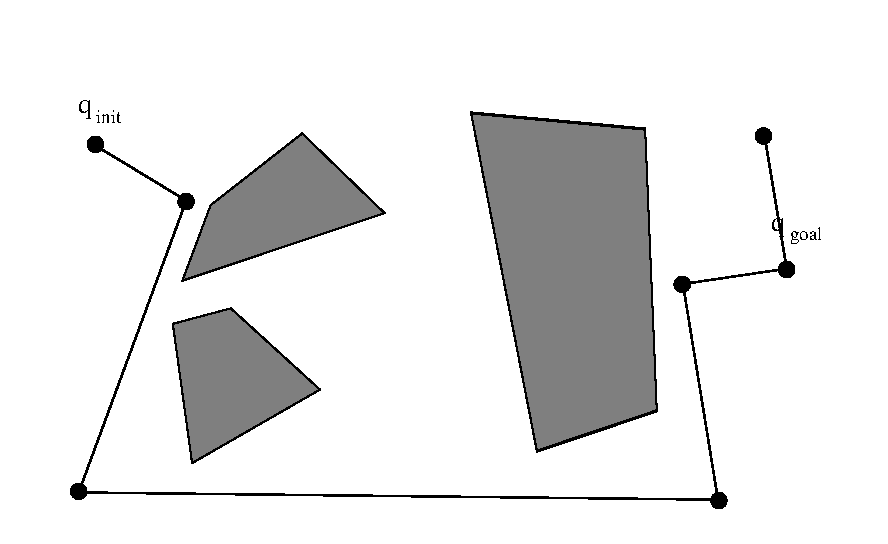
\includegraphics[width=.8\linewidth]{figures/RRT15.pdf}
}
\end{frame}

\begin{frame} {Rapidly exploring Random Tree (RRT) 2000}
\centerline {
  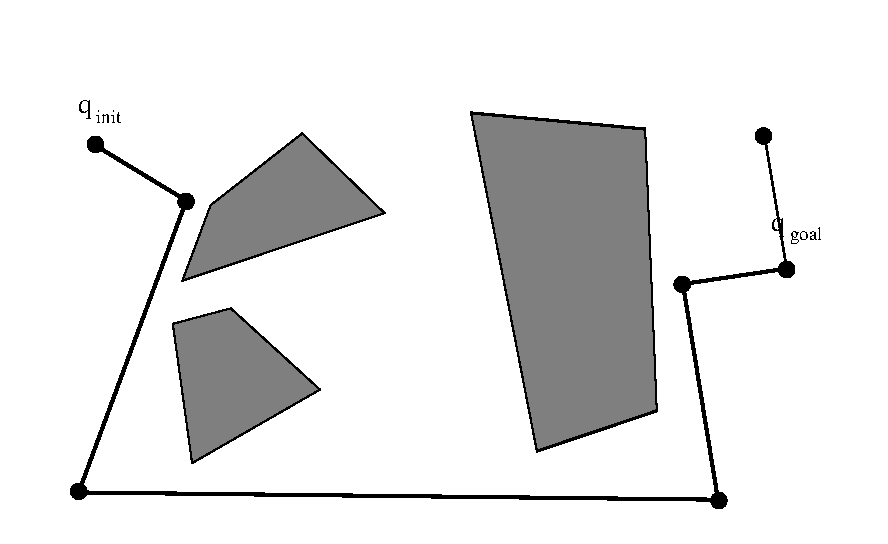
\includegraphics[width=.8\linewidth]{figures/RRT16.pdf}
}
\end{frame}

%
% random methods
%

\begin{frame} {Random methods}
  \begin{itemize}
  \item Pros:
    \begin{itemize}
    \item no explicit computation of the free configuration space,
    \item easy to implement,
    \item robust.
    \end{itemize}
    \pause
  \item Cons:
    \begin{itemize}
    \item no completeness property, only probabilistic completeness,
    \item difficult to find narrow passages.
    \end{itemize}
    \pause
  \item Requested operators~:
    \begin{itemize}
    \item Collision tests
      \begin{itemize}
      \item for configurations (static),
      \item for paths (dynamic)
      \end{itemize}
    \end{itemize}
  \end{itemize}
\end{frame}
